\documentclass[12pt]{article}
\usepackage{algorithm2e}
\usepackage{amsmath}
\usepackage{amssymb}
\usepackage{mathtools}
\usepackage{graphicx}
\usepackage{svg}
\usepackage{caption}
\usepackage{float}
\usepackage[utf8]{inputenc}
\usepackage{geometry}
\usepackage{multirow}
\usepackage{listings}
\usepackage{xcolor}
\usepackage{fancyvrb}
\usepackage{longtable}
\usepackage{polski}
\geometry{a4paper, margin=1in}

\title{Rozwiązanie Listy 3 z Metod Optymalizacji}
\author{Mikołaj Krupiński}

\begin{document}

\maketitle

\section{Opis problemu}

Na tej liście rozważany jest problem szeregowania zadań na niezależnych maszynach z kryterium minimalizacji długości uszeregowania.

Dla każdej instancji problemu dany jest zbiór zadań $[J]=\{1,\dots,J\}$, zbiór maszyn $[M]=\{1,\dots,M\}$ oraz dla każdej pary $i \in [M], j \in [J]$ dany jest $p_{ij}$, czyli czas wykonania zadania $j$ na maszynie $i$. Celem jest znalezienie takiego przyporządkowania zadań do maszyn, by całkowity czas wykonania wszytskich zadań był jak najmniejszy.

\section{Idea algorytmu}

Do rozwiązania problemu używany jest algorytm aproksymacyjny, który zwraca rozwiązanie o koszcie nie większym niż 2-krtotność kosztu rozwiązania optymalnego.

Algorytm opiera się na relaksacji instancji programowania całkowitoliczbowego przedstawionej poniżej do programowania liniowego.

\begin{align*}
    \text{minimize} && t && && \\
    \text{subject to} && \sum_{i \in [M]} x_{ij} = 1 && \forall j \in [J] && \\
    && \sum_{j \in [J]} x_{ij}p_{ij} \leq t && \forall i \in [M] && \\
    && x_{ij} \in \{0,1\} && \forall i \in [M], j \in [J] &&
\end{align*}

Przy użyciu przeszukiwania binarnego znajdowana jest liczba $T$, która jest najmmiejszym górnym ograniczeniem na całkowity czas wykonania wszytskich zadań dla instancji programowania liniowego. $T$ szukane jest w zakresie $[\frac{\alpha}{M}, \alpha]$, gdzie $\alpha$ jest czasem zakończenia wszytskich zadań dla algorytmu zachłannego.

Dla znalezionego $T$ model jest rozwiązywany. Wszystkie zmienne mające wartości całkowite są przenoszone na przydział zadań. Dla zadań nieprzydzielonych w ten sposób tworzony jest graf dwudzielny zadań i maszyn, w którym pomiędzy zadaniem a maszyną jest krawędź, jeśli zmienna odpowiadająca tej parze zadania i maszyny ma dodatnią wartość.

W tak powstałym grafie przydział zadań odbywa się na podstawie znalezienia doskonałego skojarzenia. W pierwszej do skojarzenia są dodawane liście. Każdy liść reprezentuje maszynę, więc zadanie z nią połączone jest od razu na nią przydzielane. Po usunięciu wszystkich liści w grafie pozostają jedynie cykle parzystej długości. Dla każdego z nich przydział odbywa się tak, by wybierane krawędzie tworzyły doskonałe skojarzenie.

\section{Wyniki i interpretacja}

% TODO opisać bardziej szczegółowo zbiór testowy

Wyżej opisany algorytm został zaprogramowany w języku \texttt{Julia}. Uruchomiono go dla przykładów testowych załączonych do listy. Dla każdej grupy instancji testowych w tabeli \ref{tab:error} znajduje się najmniejszy, największy oraz średni błąd, a na wykresie \ref{fig:error_plot} są błędy dla poszczególnych przykładów.

Błąd jest ilorazem wartości zwróconej przez algorytm i wartości optymalnej. Dla niektórych przykładów nie jest znana wartość optymalna z powodu przekroczenia limitu czasu wykonania solvera, stąd może wystąpić błąd mniejszy niż 1. Modelowo błąd powinien się mieścić w przedziale $[1,2]$.

\begin{table}[H]
    \centering
    \begin{tabular}{|c||c|c|c|}
        \hline
        Nazwa instancji & Minimalny błąd & Średni błąd & Maksymalny błąd \\
        \hline
        U(1,100) & 1.0128 & 1.3663 & 1.9375 \\
        \hline
        U(100, 120) & 1.0015 & 1.0844 & 1.505 \\
        \hline
        U(100, 200) & 1.0038 & 1.0885 & 1.5024 \\
        \hline
        U(10, 100) & 1.0052 & 1.1385 & 1.5357 \\
        \hline
        U(1000, 1100) & 0.9999 & 1.0835 & 1.4993 \\
        \hline
        JobsCorre & 1.0088 & 1.1863 & 1.8269 \\
        \hline
        MaqCorre & 1.0076 & 1.2549 & 1.8824 \\
        \hline
    \end{tabular}
    \caption{Tabela zakresów błędów dla poszczególnych instancji testowych}
    \label{tab:error}
\end{table}

\begin{figure}[H]
    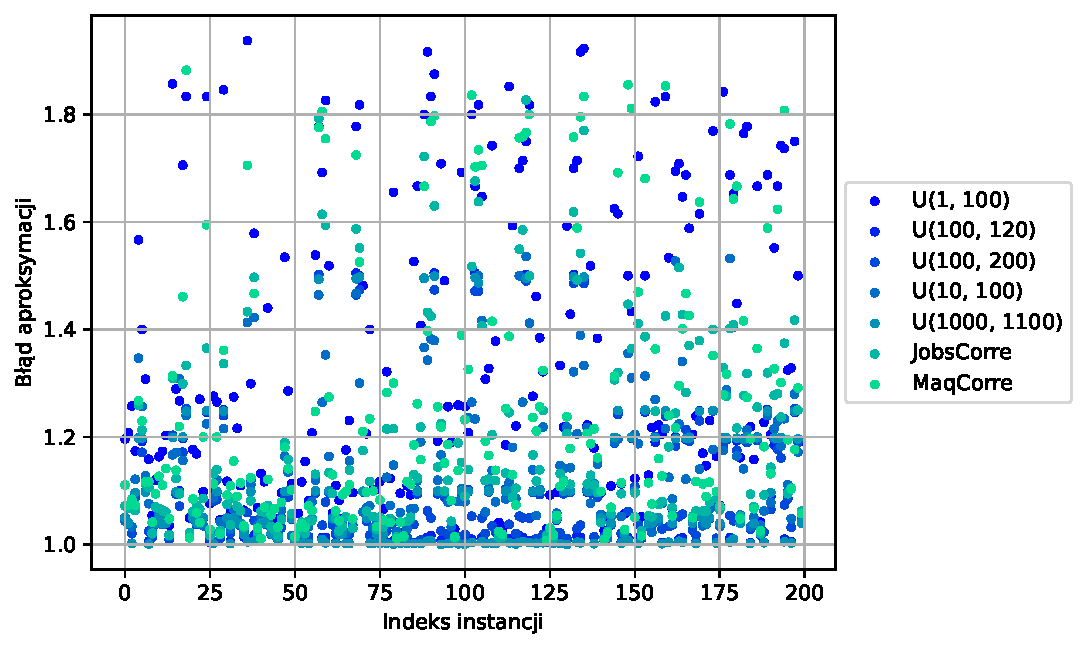
\includegraphics[width=\textwidth]{error_plot.pdf}
    \caption{Wykres błędów dla poszczególnych instancji testowych}
    \label{fig:error_plot}
\end{figure}

Żadna ze zwróconych wartości błędu nie przekracza 2, co jest zgodne z teoretycznym założeniem algorytmu. W wielu przypadkach wartości błędu są bliskie 1, a średnie nie przekraczają 1.4, co sugeruje, że algorytm zwraca rozwiązania bliskie optymalnym.

\end{document}